\chapter{Path Computation Techniques for Inter-domain LSPs}
\label{cha:PathCompTechniques}
\markright {Path Computation Techniques for Inter-domain LSPs}

\section{Introduction}
Path computation in large, multi-domain, multi-region, or multi-layer networks has become more complex and demanding in terms of CPU resources. With the wide deployment of GMPLS and the variety of switching technologies such as packet, TDM and wavelength switching, path computation constraints have increased and have become more stringent than simple bandwidth availability or administrative constraints in packet-switched networks. For example, the path computation of diverse paths in a multilayered network may involve diversity be satisfied with respect to all underlying switching layers (\eg packet, wavelength, fiber, duct, etc, \dots). In addition, as MPLS TE becomes the preferred choice for network operators, and with the rise of Point-to-Multipoint TE (\gls{P2MP-TE}), the computation of remerge-free P2MP paths to a high number of destinations is also becoming a challenge. Therefore, supporting these complex computation problems-- when even heuristic algorithms are computationally intensive-- at every network node becomes an expensive and sometimes infeasible solution.

Inside an AS composed of a single IGP area, all \gls{LSR}s learn the complete topology of the network by means of link-state flooding \gls{IGP} protocol such as ISIS or OSPF. Each \gls{LSR} is able to compute the complete path from head-end to tail-end node for the LSP. However, the topology of an AS is hidden from LSRs that lie outside of that AS, notably for confidentiality purposes. As a consequence, an LSR is not able to compute an end-to-end path for an LSP crossing multiple ASes. Therefore, the computation of such a path has to be distributed among multiple nodes, where each node computes a sub-segment of the path based on its own knowledge of the local domain topology as well as global domain reachability information provided by inter-domain routing protocols (\eg BGP).

In this chapter, we investigate the different approaches to distributively computing such end-to-end paths LSPs that cross multi-area or carrier networks. We present the current state of development of two distributed techniques for the computation of paths respecting QoS requirements together with a centralized technique that we use in subsequent chapters as a reference point to compare with the other techniques. In appendix A, we present our implementation of these techniques in a simulator.

\section{Overview of TE LSP Spans}
In this section, we examine the issues involved in selecting a suitable path for \gls{TE}-LSPs that:
\begin{itemize}
	\item lie within the boundary of a single \gls{IGP} area (also known as intra-area TE LSPs),
	\item traverse inter-area boundaries \ie their path spans multiple \gls{IGP} areas owned by the same carrier  (also known as intra-carrier, inter-area TE LSPs), or
	\item traverse inter-carrier boundaries \ie their path spans multiple carriers domains (also known as inter-AS TE LSPs)
\end{itemize}
Examples of these types of path are shown in Figure~\ref{fig:IntraInterAreaCarrier}.

\begin{figure}[t]
\centering
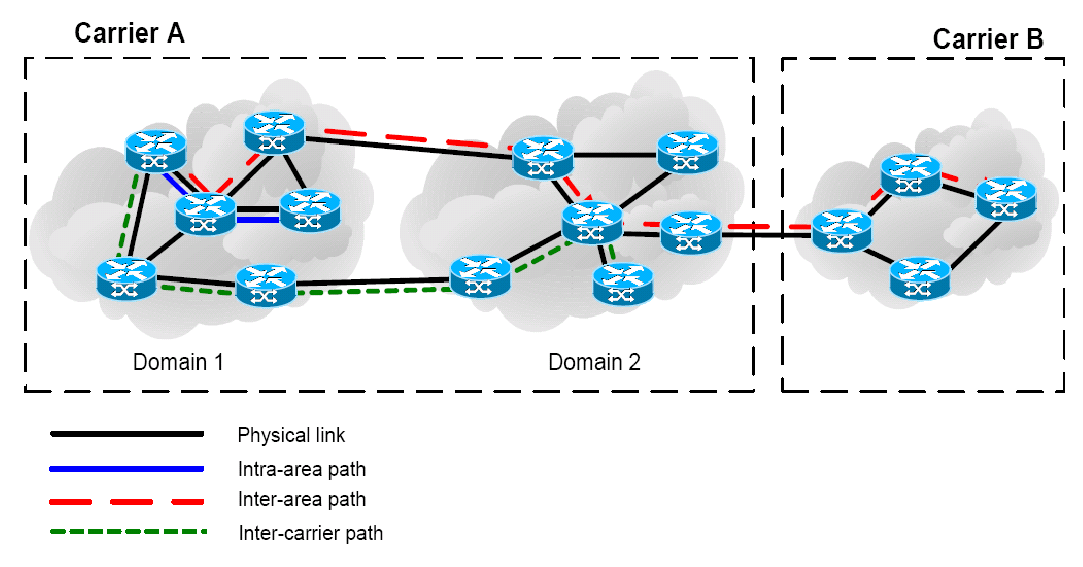
\includegraphics[scale=0.7]{Figures/IntraInterAreaCarrier.eps}
\caption{Intra-area, Inter-area and Inter-carrier paths}
\label{fig:IntraInterAreaCarrier}
\end{figure}

\subsection{Intra-area TE LSPs}
It is relatively straightforward to select a path for an LSP if the ingress and egress points lie within the same IGP area.  The information disseminated by the IGP allows each node to build-up a database of every link in its local area and the appropriate \gls{TE} properties associated with them. If a node receives a request to set up an \gls{LSP} that must meet a certain set of \gls{TE} constraints, then this database can be used to calculate a suitable, complete, explicit least-cost path through the area to the specified egress point of the LSP. If required, the ingress \gls{LSR} can also calculate a diverse backup route (\eg a route that does not use the same link or node) at the same time to provide additional reliability for the LSP.

Typical information flooded by IGPs within a TE-area includes link's: 
\begin{itemize}
	\item maximum bandwidth,
	\item maximum reservable bandwidth: aggregate, per class, and/or per LSP connection
	\item administrative weights (\eg IGP and TE costs),
	\item the Shared Risk Link Group (\gls{SRLG})
	\item delay or latency, and
	\item other characteristics such as resource class attribute color, link availability, \etc
\end{itemize}

As LSPs are established and torn-down, the above \gls{TE} characteristics (such as the available bandwidth) associated with links traversed by the LSPs change dynamically. The IGP, therefore needs to continuously update other LSRs in the same area about the state of their connected links.  To avoid this from happening frequently and causing churn, LSRs could define longer periodic flooding timers. Simultaneously, resource thresholds (\eg available bandwidth) can be set to trigger immediate flooding only when crossed. In this case, if a LSP connection is rejected at any LSR along the LSP path (\eg due to stale resource information at the time of computation of the LSP path), the LSR that blocks the LSP will also immediately trigger flooding of the link state so all other LSRs in the domain can synchronize their TED with recent information.

\subsection{Inter-area TE LSPs}
There are several reasons to divide a single carrier network into multiple areas, including the scalability of the IGP protocol used, administrative convenience, business structure, and compatibility or inter-operability among different vendor equipment.

Unlike the intra-area case, if the LSP must traverse multiple areas, the ingress point of the LSP does not know the details of every link and/or node that could be traversed by the LSP. Since the IGP only runs within a given area, it does not distribute topology information about all the links the LSP might traverse. The information provided by the IGP can no further be used to compute the path up to the Area Border Router (\gls{ABR}) within the area.

However, without this full knowledge a node cannot reliably choose the ``best'' route for an LSP to take-- typically defined as the least cost path that satisfies the constraints associated with the LSP. Instead, the node must try to approximate this function. The goal is to select a path that with high confidence that satisfies the specified constraints without incurring an unacceptable cost in terms of complexity and/or scalability. Generally, there are two ways in which a node can attempt to provide this function.

\subparagraph{Push mechanisms}
\label{par:PushMechanisms}
In these cases, an inter-area routing protocol pushes down a summary of information about all other areas to the nodes in each area. In Chapter~\ref{chap:HierarchyRTAggregation} we discuss in more details how such summary can be formed so nodes obtain a limited or summarized view of the network outside of their own area.

\subparagraph{Pull mechanisms}
\label{par:PullMechanisms}
When using pull mechanisms, nodes do not need to maintain a view of the rest of the network. Instead, when they receive an LSP set up request, they query a remote entity that has a better global view of the network. This entity can further query other sources to collaboratively assist in finding the end-to-end path. On receiving a response to the query, the entity provides the node with a path to the destination that. The \gls{PCE} framework described in Section is one example of this approach. Moreover, In Chapter~\ref{chap:ServiceGuarTE} we propose a novel scheme that falls under this approach that can provide.

Furthermore, there are other complications to setting up protected LSPs spanning different areas. Due to lack of knowledge of all nodes and links along the LSP's working path, it is a challenging tasks for ABR LSR nodes that perform the sub-path computation to find backup LSP paths that protect against node or link failure. In Chapter~\ref{chap:ServiceGuarTE}, we present a mechanism to collect and furnish such information to nodes along the LSP path that would make use of it to compute the such diverse backup paths.

\subsection{Inter-carrier(AS) TE LSPs}
If multiple carriers operate within the network, a single organization will not be responsible for administering the entire network. In order to meet customer requirements, carriers may need to negotiate and provision resources across other carrier's network. The following issues will arise when doing so.

\subparagraph{Issues of Trust}
\label{par:IssuesOfTrust}
When different carriers administer networks, it is critical that a carrier does not disclose sensitive internal information about their topology to other neighboring carriers who may be competitors and can potentially employ the information to gain competitive advantage. For example, carriers may be reluctant to disclose details of the bandwidth available within their network or whether their topology allows them to protect a particular LSP. This makes it much harder to design an efficient path computation algorithm that can calculate paths that span multiple carriers. Also, if a carrier discloses too little information, traffic may sometimes end-up avoiding that carrier network due to the inaccuracy and/or inadequacy of disseminated information which can ultimately  have negative commercial implications.

\subparagraph{Protection issues, standardization and SRLGs}
\label{par:ProtectioIssues}
Setting up a fully protected, end-to-end LSP across multiple carriers is particularly difficult. Nevertheless, ensuring that two LSPs use links in completely different two areas or even different carrier networks does not necessarily guarantee that failure diversity  for the LSP. As different links may use the same physical conduit-- for example different optical fibers may share the same cable and consequently  share the same fate.

To solve this, the Shared Risk Link Groups (SRLGs) can be introduced within the carriers networks. In this case, different links within the carrier network may be grouped together as belonging to a particular SRLG. However, links owned by different carriers can still share the same lower layer infrastructure network(\eg physical conduits). Hence, the concept of SRLG still needs to be extended for the inter-carrier environment to enable nodes across all areas/domains to be able to understand which SRLG is being referred to-- \ie SRLG identifiers need to be standardized across the whole network. This, however, is challenging especially in the inter-carrier environment. A key issue is how to compute paths across multiple areas and/or carrier networks that satisfy the specified constraints.  
In Chapter~\ref{chap:HierarchyRTAggregation} we present a scheme suitable for the inter-area or carrier environment that embeds SRLG information in hierarchical Aggregate Link Resource Tree (ALRT) that is subsequently disseminated to other areas/domains. ABRs, then, can distinguish between links belonging to different SRLGs and compute diverse paths that avoid links of same SRLG.

\section{Inter-domain Path Computation Schemes}
Path computation for end-to-end paths across multiple domains or layers is the next step towards wide-scale deployment of a distributed control plane that supports TE. In this section, we describe three major approaches to path computation for inter-domain LSPs, namely, the IP shortest path, the per-domain path computation, and the PCE-based path computation.
 
\subsection{Inter-domain IP Shortest Paths}
The simplest technique to establish an inter-domain TE LSP is for the LSP path to follow the IP shortest hop-by-hop path. Using this scheme, the RSVP Path signaling messages used to signal the LSP are routed at each hop by performing a IP route lookup for a preferred next-hop (\eg using the IGP routing table for intra-area nodes, or the BGP routing table for destinations outside the AS). Note, this path is usually chosen by Label Distribution Protocol (LDP) LSPs when used between ASs. The drawback of this scheme is that these shortest paths may become overloaded or may not respect the requested QoS constraints.

Figure 4.1 shows the IP forwarding path from node S to node D. This path crosses nodes S-R11-R12-R21-R23-R41-D. More precisely, S determines that R21 is the BGP NH to reach nodes belonging to prefix D/16, based on its forwarding table. From its forwarding table, S also knows that R11 is on the shortest path to R21. Thus, it sends IP packets to R11. The same process takes place at each path on the forwarding path, until the destination is reached.

We note that the end-to-end delay along the IP forwarding path is equal to 115ms. Thus, it could not support a flow requiring a lower delay bound although there might exist other paths (\eg going through S-R11-R14-R31-R32-R41-D, respecting this end-to-end delay constraint. However, this path is not available at node S.

\subsection{Per-domain ERO expansion}
The per-domain path computation scheme defines a technique for establishing inter-domain LSPs where the path is computed during the signaling process on a per-domain basis. It is notably a combination of the inter-domain IP shortest path computation heuristic, and the intra-area path expansion scheme.

The per-domain path computation is applicable when the full ``strict path'' of an inter-domain LSP path is not pre-determined prior to initiating the signaling of the LSP. This usually arises from the lack of TE topology visibility of neighboring TE domains when network state information is not exchanged across domain boundaries. In this case, a set of (loose and strict) hops can be either statically configured at the head-end LSR or dynamically computed at signaling time.


Inside RSVP-TE, it is possible to indicate the path or a portion of the path to be followed by the LSP inside an object called the Explicit Route Object (\gls{ERO}). The ERO expansion technique relies on this object and consists of completing, at the entry ABR of a domain, the path computation up to the next IGP or BGP hop, i.e. last reachable hop toward the destination. This node is usually either the first hop inside the downstream domain or the last hop inside the current domain. The computed path segment is then stored inside the ERO of the RSVP-TE Path message and the message is forwarded along the path inside the ERO. Upon receiving the RSVP Path signaling message, an \gls{ABR} or \gls{ASBR} along the TE LSP path performs a loose hop expansion or partial route computation in its own domain to reach the next loose hop A(S)BR before forwarding the path message downstream.

It is worth noting that such path computation technique does not always guarantee finding a feasible constrained path since it relies on heuristics to choose an appropriate NH among the available NHs announced for the destination (e.g. among the BGP preferred next-hops).  Furthermore, it cannot be efficiently used to compute a set of inter-domain diversely routed TE LSPs. For example, a head-end LSR computes a set of strict path hops up to the first ABR visible in its TE database (TED) topology and then appends the path with loose hops for boundary or domain exit nodes in remote domains. When dynamically computed, the loose hops can be learnt through discovery mechanisms such as IGP, BGP, or policy routing information.

The ERO expansion technique can also make use of the crankback capability of RSVP-TE to stop the establishment of an LSP when a node cannot compute a path toward the destination and attempt different Next Hop (NH) ABR. The ABRs can store the list of NHs that have already been tried for an LSP and lead to an unfeasible path with regard to the constraints. When no NH is found that can complete the path with a segment respecting the constraints, a ``crankback'' is performed by generating an RSVP Path Error message and sending it upstream. The upstream ABR in turn will attempt the expansion of a new segment avoiding the NHs that have already been tried.

As such, the role of crankback is important for the establishment of inter-domain LSPs when only limited information about remotely connected domains is available. If a bad choice is performed by the heuristic at any ABR, a downstream ABR may not be able to complete the computation of the path. Crankbacks enable to cope with such a situation and subsequently try alternative NHs.
 
Figure~\ref{fig:CentralizedPce} illustrates the RSVP-TE ERO expansion technique with path computation that takes place at ABRs. In this example, an LSP with delay constraint of 100 ms has to be established from S to D. Therefore, the source of the LSP $S$ sends out a Path signaling message to $D$. Inside this message (a), the source specifies the tail-end and the constraints of the LSP. When the ABR receives the Path message, it attempts to expand the a path segment respecting the constraints based on its knowledge of the internal topology and the BGP routes for the destination. Then, it forwards the Path message along the computed path segment. 

At the ingress \gls{ASBR} inside AS2, R21, the process described in the previous paragraph is repeated. However, PCE2 is not able to provide a path segment that respects the constraints. The only way, known by PCE2, to reach D is via the NH R41. However, this requires to use link R23-R41. Since this link has a longer delay than the delay constraint for the remaining LSP�s segment, PCE2 cannot return a path segment that respects the constraint to R21. Thus, PCE2 sends back to R21 a PCRep that indicates this situation. Consequently, crankback occurs at R21.

R21 sends a Path Error message upstream. When the Path Error message arrives at S, S sends a new PCReq to PCE1. This request (b) contains in addition to the constraints in PCRep (a), the address of the NH that lead to an infeasible path, R21. PCE1 provides a path segment that ends at NH R23. This NH is also a bad choice. S sends a Path message along the path segment toward R23 and is notified of the failure to continue the establishment of the LSP after crankback occurs at R23 because there is no BGP NH, known by PCE2, reachable with a segment that respects the specified delay constraint.

Upon reception of the Path Error message, S sends PCReq (c) to PCE1 with the constraint to avoid both R21 and R23. PCE1 replies with path segment ending at NH R31 in PCRep (c). A Path message is sent by S along the computed segment. The ingress ASBR, R31, in the downstream AS, AS3, asks its PCE, PCE3, for the computation of a path segment starting at R31 and ending at the entrance inside a downstream AS. PCE3 replies with path segment R31-R32-R41. This path segment is inserted inside the ERO of the Path message and the establishment of the LSP continues until the LSP�s tail-end is reached.

\subsection{The Path Computation Element}
The Path Computation Element (PCE) may be an \gls{LSR}, \gls{ABR}, \gls{ASBR} or any dedicated server that participates in the computation of constrained paths. A PCE is usually assigned to each domain and can compute constrained paths segments within its domain. Paths computed by individual PCE are usually referred to ``local'' path segments. The PCE can also compute an end-to-end path based on the local path segment as well as path segments received from other PCEs. When the head-end and the tail-end of the LSP do not belong to the same domain or, if the LSP has to cross different domains, computation of the path of the LSP is distributed, and multiple PCEs may contribute to the computation of the end-to-end path.

The domain of a PCE may span a single or multiple areas, AS or multiple ASes-- with at least one PCE in each AS. For clarity reasons, we describe the following path computation techniques based on the existence of a single PCE inside each AS. However, they are also applicable (1) when multiple PCEs exist inside ASs with domain covering an AS (\eg AS confederations) as well as (2) when the ASs are divided into more than one IGP area.

The PCE computes path segments respecting given QoS and diversity constraints based on its own TED. The content of the TED depends on the domain of the PCE and contains at the least the topology of the domain and the TE attributes for links belonging to the domain. In addition, it may contain the TE attributes of the links at the border of the domain, for example the inter-AS links.

Moreover, the PCE needs to know about reachability information for destinations outside the domain of the PCE. This information is distributed by the BGP for external prefixes outside the AS. Nodes requesting a path computation from a \gls{PCE} are referred to as Path Computation Clients (\gls{PCC}). Thus, a PCE asking for a computation from another \gls{PCE} acts as a \gls{PCC}. The Path Computation Engine Protocol (\gls{PCEP}) is the communication protocol used between \gls{PCC}s and \gls{PCE}s. A message sent by a \gls{PCC} to a \gls{PCE} requesting a path computation is referred to a PCReq. The response of the PCE to the PCC is a Path computation Reply, PCRep.

An additional mechanism, called PCE discovery, is required in order for the PCCs to learn the list of available PCEs in their domain and in neighboring domains. In Chapter~\ref{chap:EvaluationPCESelectionSchemes} we present an evaluation of different PCE selection schemes as well as present novel heuristic to selecting the preferred PCE among available ones.

\begin{figure}[t]
\centering
\includegraphics[scale=0.8]{Figures/CentralizedPce.eps}
\caption{Centralize computation with a global PCE}
\label{fig:CentralizedPce}
\end{figure}

\subsubsection{Centralized PCE Path Computation}
Using this technique, the computation is performed by a single entity, that we call ``global PCE''. The domain of the global PCE covers all the domains crossed by an LSP. We assume that the global PCE learns the complete topology by receiving the link state updates from each domain. The global PCE performs as a path computation for each LSP. The algorithm used by the global PCE for path computation is the CSPF algorithm, in this thesis. This CSPF computation by a global PCE provides an indication of the path quality that can be achieved with a centralized computation.

Such a centralized solution could be envisaged when MPLS LSPs are entirely contained within ASes that belong to the same company (\ie intra-carrier case). However, it is not realistic for LSPs that cross ASs from different companies (inter-carrier LSPs) as this requires the ASs to cooperate and reveal their internal topology. As well, this solution also exhibits scalablility issues with the number nodes and links of subscribing ASes. We use this scheme as a benchmark and compare it with our proposed techniques.

In Figure~\ref{fig:CentralizedPce}, we assume that the domain of the PCE covers AS1, AS2, AS3, AS4 as well as their interconnections. When an LSP is required between the head-end $S$ and the tail-end $D$, $S$ sends a PCReq message to the PCE. The constraints required for the LSP are specified in this message. Upon reception of the PCReq, the PCE computes a path that respects the constraints. Then, it sends the path back to the PCC, $S$ in a PCRep message. Here, we see that the path returned by the PCE is the path with shortest delay because the PCE uses the CSPF algorithm.

\subsubsection{Cooperative PCE Path Computation}
A cooperative PCE communicates with other PCEs in order to request or delegate the computation of path segments contained in domains or regions for which it does not possess enough topological information. As mentioned earlier, a cooperative PCE asking for a path computation from another PCE is considered as a PCC.

Using this technique, a PCReq message specifying the constraints for the LSP is relayed from the PCE of one domain to the PCE of downstream domains. Upon reception of the PCReq, the PCEs in downstream domains run a path computation technique to attempt finding path segments starting from the domain ending at the tail-end of the LSP. These segments are sent to the upstream PCE inside a PCRep message.

One such path computation technique, called Backward Recursive PCE-based Computation (\gls{BRPC}) [XXXX] was designed to find the shortest path for a constrained inter-AS LSP makes the assumption that the list of domains to be crossed by the LSP is known prior to the computation. Thus, the computed path is the best path that can be obtained along this inter-domain path. Such assumption is usually applicable in the inter-area case where areas to be crossed by the LSPs are known prior to the computation of the path. This is since an AS is usually divided into a backbone area and stub areas connected to the backbone. The path between two stub areas always goes from the area of the head-end LSR to the backbone area and ends in the area of the tail-end LSR.

However, The above assumption concerning the knowledge of the domains to be crossed by the LSPs holds true if each domain corresponds to an area. However, ASs to be crossed by a constrained inter-AS LSP cannot be known in advance. In Chapter~\ref{chap:ServiceGuarTE} we present a novel scheme that extends the cooperative PCE path computation techniques to finding the list of domains to be crossed by a QoS constrained LSP so suitable PCEs  residing in each can be consulted for path segment calculation.

Figure 4.4 illustrates the computation of inter-AS constrained paths by means of cooperative PCEs. We assume that the list of domains to be crossed by the LSP is not known a priori contrary to [VZB06]. Thus, the PCEs contact a PCE in each downstream domain available from the TED, in order to find the shortest path for the LSP. As a consequence, the optimality of the path found for the LSP depends on the content of TED. Here, we assume that the TED of a PCE is composed of all the BGP routes learned inside the AS6. In general, the TED could be populated
by other means than with BGP. However, a PCE has to be able to determine a set of possible downstream domains from the TED and to contact the PCEs that are discovered inside these domains. The LSP to establish is subject to a maximum delay constraint of 100ms. The head-end of this LSP is router S in AS1. The tail-end of the LSP, node D, belongs to AS4. The longest matching prefix advertised for D is D=16. The central part of the figure shows the physical topology of the ASs and their interconnections. In the top part of the figure, we see the PCEs of each ASs, labels for the messages exchanged between PCEs and the BGP routes known by the PCEs. The content of the messages exchanged between PCEs is shown at the bottom of the figure.

The head-end of the LSP, S sends a PCReq message to the PCE of its AS, PCE1. PCE1 in AS1 has three routes for prefix D=16. We observe from the
AS-path that two of these routes are received from AS2, with two different BGP Next-Hops (NHs) and the other route is received from AS3. Thus, it sends a PCReq message to PCE2 and PCE3, the PCEs inside AS2 and AS3. The PCReq messages contain the address of the tail-end of the LSP and the constraints for the LSP. The delay constraint is not necessary because the output of the computation technique is the shortest delay path. If the delay of the path returned to the LSPs head-end is above the delay constraint, there is no suitable path for the LSP.

PCE2 and PCE3 have one route for prefix D=16. The NH for this route is router R41 in AS4. Therefore, PCE2 and PCE3 both send a PCReq to PCE4.
PCE4 computes a path segment from R41 to D, the tail-end of the LSP. Then, it sends the segment with its delay in PCRep messages (5) and (6) upstream to PCE2 and PCE3, respectively. When PCE2 receives PCRep (5), it has the response to the single PCReq that it sent for the LSP. It has all the requested information. Thus, it is now able to compute path segments from the entrances inside its domain to the destination of the LSP or to determine that is such path segments respecting the requested constraints cannot be provided. For this purpose, the PCE performs a SPF computation on the graph composed of the local topology, the inter-AS links and the segments received from the downstream PCE. The result is two path segments starting at nodes R21 and R23, ending at D. Upon reception of PCRep (6), PCE3 performs the same actions as described for PCE2.

Next, PCE2 sends the resulting segments and their delays inside PCRep (7) to PCE1. In addition, PCE3 sends path segment from R31 to D and the delay of the segment to PCE1, in PCRep (8). Because PCE1 received replies from all the PCEs it sent PCReq messages to, it computes the end-to-end path based on the local topology, the inter-AS links connected to AS1 and the received segments. The resulting path is S-R11-R14-R31-R32-R41-D with delay of 16ms.

This path is sent in PCRep (9) to the head-end of the LSP, S. Finally, S initiates the establishment of the LSP along this path. For this purpose it stores the list of nodes along the computed path inside the ERO. Thus, the RSVP Path message follows the computed path and the LSP is established along this path.

In order to respect the confidentiality requirement of SPs (see section 3.4), PCEs may return path keys [BVF06] inside PCRep messages, instead of returning path segments that reveal sequences of hops inside their domains. A Path Key Sub-object consists of a key that replaces the Confidential Path Segment (CPS) generally contained inside the domain of the PCE and of the identifier of the PCE.
Path Key Sub-objects (PKS) can be stored inside the ERO of the RSVP Path messages. Such sub-object must follow the node responsible for expanding the path key, that is the first node of the confidential path segment. This node sends the path key to the PCE with identifier contained in the PKS for expansion of the path key into a sequence of nodes.

In section A.4 of appendix A, we provide a detailed description of our implementation of this technique. We implemented this technique in parallel to the elaboration of BRPC [VZB06] at the IETF. Thus, our implementation differs from BRPC in matters that were not described at the IETF at the time of our implementation.

Moreover, our implementation solves certain issues that have not yet been considered at the IETF.We show in appendix A that these divergences do not have an impact on the resulting computed paths. However, they induce differences on the information and number of messages exchanged between cooperative PCEs. In the next paragraphs, we give a brief overview of these differences. A more detailed description is provided in section A.4.2 of appendix A. The first difference is that, in our implementation, we do not assume that the list of domains to be crossed by an LSP is known prior to the computation of its paths.

It results that all the PCEs that are downstream of the current PCE on the path to the LSP�s tail-end need to be contacted if the optimal path to the destination has to be found. This difference implies that a PCE may receive multiple requests (PCReqs) for the same LSP. These requests may have crossed a different list of upstream PCEs. Our implementation has to distinguish such PCReqs from PCReqs that are looping. A looping PCReq results in the generation of a Path Computation Error (PCErr) message. The other PCReqs should trigger a PCReq message as reply.

Because PCEs may receive multiple requests for the same LSP, they may benefit from maintaining a cache in order to avoid recomputations and to reduce the exchange of messages with other PCEs. In our implementation, we distinguish two types of PCEs. Stateless PCEs do not maintain a cache with the computed path segments and the responses from the downstream PCEs contacted before, for an LSP. These PCEs need to recompute the local paths segments and to contact all the downstream PCEs each time a PCReq is received. On the contrary, stateful PCEs maintain a cache for each LSP. This cache contains the local paths computed for the LSP and the responses from the downstream PCEs that were contacted for
the previous requests. A stateful PCE does not need to recompute already known local path segments. Moreover, it only sends PCReq messages to the PCEs that did not participate in previous computations for the available NHs.
The second difference between BRPC and our implementation concerns the computation of the local path segments. In BRPC, a PCE computes the segments from its ingress ASBRs to a set of ingress ASBRs inside the downstream domains upon reception of the replies to the PCReqs that it sent. In our implementation, the local path segments are computed on receipt of a PCReq message. We show in section A.4.2 of appendix A that this difference has an impact on the number of messages exchanged during the computation of interdomain paths. In certain cases, BRPC requires fewer messages to be exchanged while in others fewer messages are exchanged with the technique that we implemented.

In section A.4, we describe the algorithm that we use for the computation of the lower and upper bounds on the number of messages that are exchanged in the computation of each LSP with our implementation of cooperative PCEs. The number of messages exchanged for the computation of a particular LSP with our implementation of cooperative PCEs is comprised between these bounds. This number approaches the upper bound if the PCEs are stateless. The number of messages exchanged between cooperative PCEs approaches the lower bound if all PCEs are stateful and maintain the content of their cache during an infinite period of time. The lower bound is also a lower bound on the number of messages exchanged with BRPC. However, we show in A.4.2 that the upper bound on the number of messages with BRPC may be higher than the upper bound computed
for our implementation with algorithm 4.

TSAAD: we need simulations on IP forwarding, ERO expansion and PCE path computation��..

\section{Problem Definition and Formulation}
\subsection{TE Problem Definition}
The problem of concern, hereafter denoted by the TE problem (TP) for short, entails minimizing the overall path cost (\eg typical costs that are considered are IGP or TE cost, or  aggregate transmission delay) over all data flows, each of which is subject to constraints on the link bandwidth capacity. The TP is similar to the restricted-shortest path problem (RSP) [], a NP-complete problem whose goal is to find a shortest path that does not violate a resource constraint. To not violate the constraint, LSPs would tend to be configured along paths that could be longer than the shortest ones, potentially incurring higher costs (\eg higher end-to-end transmission delays, \etc). Thus the minimization of the total cost is pertinent, whereby shorter paths are favored so long as they do not violate the bandwidth constraints. The problem formulation assumes that the data flows and LSPs are one-to-one related. The routing problem is formulated as an integer-programming problem, whose objective function amounts to minimizing the overall cost in all of the links, and whose constraints prevent the violation of the link-bandwidth limits as well as impose the connection-oriented transmission of the MPLS architecture.

In MPLS terminology connections are set-up between an ingress-egress pair of routers. Each connection request arrives at an ingress router
which determines the explicit route for the LSP according to the current topology and to the available capacities at the IP layer. It is assumed that every router runs a link state routing protocol with extensions for link residual bandwidth advertisements.

A connection request $i$ is defined by a triplet $(i_i, e_i, b_i)$, where $i_i$ and $e_i$ specify the ingress and egress routers and $b_i$ indicates the amount of bandwidth required. In the rest of the chapter we will consider only the routing of bandwidth guaranteed connections.

The corresponding LSPs will be routed through the network and, at each instant, one determines the virtual load of a link by summing the bandwidth $b_i$ of the connections passing through the link. The difference between the \textit{link capacity} and the \textit{virtual load} gives the \textit{residual bandwidth}. The \textit{minimum residual bandwidth} over all links of a network is called the \textit{available capacity of the network}. This value identifies the most congested links.


\subsection{Intra-domain TE Problem Formulation}
Consider a single domain IP/MPLS network which consists of LSR nodes and TE links connecting them. Let $\mathcal{N}$ denote the set of LSR nodes and $\mathcal{L}$ the set of TE links of the network. We denote by $l_{ij}$ a link from node $i$ to node $j$. The network topology can be modeled as a directed graph $G=(\mathcal{N},\mathcal{L})$, where $|\mathcal{N}|= n$, and $|\mathcal{L}| = m$. 

Some of the information pertinent to the network topology and links states are characterized by:

\begin{definition}{$\mu_l$}
or $\mu_{ij}$ the capacity of the TE link $l_{ij}$-- \eg the available bandwidth on $l$.
\end{definition}

\begin{definition}{$c_l$}
the cost of transmission when using link $l_{ij}$-- \eg the communication delay on $l_{ij}$.
\end{definition}

\begin{definition}{$a_l$}
the administrative cost of using link $l_{ij}$.
\end{definition}

\begin{definition}{$M_l$}
the maximum allocation multiplier or over-subscription factor of a link $l$.
\end{definition}

We denote the set of LSPs as $\mathcal{K}$. The parameters describing the LSP data flows are:

\begin{definition}{$\mathcal{K}$}
total number of LSPs, where $s_k$ and $d_k$ are the ingress and egress nodes of $LSP_{k}$.
\end{definition}

\begin{definition}{$\lambda_k$}
the bandwidth requested by $LSP_{k}$.
\end{definition}

\begin{definition}{$h_k$}
the maximum allowed number of LSR-hops through the network for a $LSP_{k}$.
\end{definition}

Given the above, the TE constraint-based routing (CBR) problem is charaterized by a set of demands (LSPs)--  described by a set of attributes-- that are to be routed through the network. The objective is to select the optimal placement of LSPs through the network while adhering to the constraints imposed. The unknown variables that need to be determined based on optimizing a certain objective function and satisfying a set of constraints.

The rate of traffic allocated by IE-pair $k$ on link $l$ is denoted by $x_l^k$:

\begin{equation}
\label{eqn:trafficRate}
x^k_l =
\begin{cases}
1, &\text{if $LSP_k \in \mathcal{K}$ is routed over link $l \in \mathcal{L}$} \\
0, &\text{otherwise}
\end{cases}
\end{equation}

The induced load $y_l$ on link $l$ is:
\begin{equation}
\label{eqn:inducedLoad}
y_l = \sum_{k_l \in \mathcal{K}} x^k_l, \quad \mbox{for all $l \in \mathcal{L}$}.
\end{equation}

Load $y_l$ on link $l$ incurs a cost $C_l(y_l)$, which is assumed to be an increasing and convex function of the load $y_l$. The objective in the unconstrained path computation problem is to minimize the total cost by choosing an optimal traffic allocation $x^* = (x^k_l ; k \in \mathcal{K}, l \in \mathcal{L}))$. The problem is formulated as follows:

Resource based optimization would lead to an objective function that minimizes the sum over all links of the product of the cost and the total flow on each link. The cost can be assumed any of the applicable additive defined costs (\eg communication delay, link-availability, \etc).

\begin{equation}
\label{eqn:min1}
Minimize \quad C(x) = \sum_{l \in \mathcal{L}} C_l(y_l)
\end{equation}

Or,

\begin{equation}
\label{eqn:min2}
Minimize \quad z = \sum_{l \in \mathcal{L}} \sum_{k=1}^{\mathcal{K}} c_l \lambda_{k} x^k_l, \qquad \mbox{for all $l \in \mathcal{L}$}.
\end{equation}

The basic set of constraints are:

\begin{equation}
\label{eqn:constraint1}
\sum_{k \in \mathcal{K}} \lambda_k x_l^k \leq \mu_l M_l
\end{equation}

\begin{equation}
\label{eqn:constraint2}
x^k_l \geq 0, \qquad \mbox{for each $l \in \mathcal{L}$ and $k \in \mathcal{K}$}
\end{equation}


\begin{equation}
\label{eqn:constraint3}
\sum_{l \in \mathcal{L}} x_l^k \leq h_k, \qquad \mbox{for all $k \in \mathcal{K}$}
\end{equation}


\begin{equation}
\label{eqn:constraint4}
\sum_{\forall l | i = s_k}  x_{il}^{k} - \sum_{\forall l | i = d_k} x_{il}^k = b_i^k, \qquad \mbox{for all $i \in \mathcal{N}$}
\end{equation}

where:
\[
b_i^k =
\begin{cases}
1, &\text{if $i=s_k$, ingress LSR for $LSP_k$} \\
-1, &\text{if $i = d_k$, egress LSR for $LSP_k$} \\
0, &\text{otherwise}
\end{cases}
\]

Constraint family (2) imposes bounds on the data traffic in each link, whereas (3) . Variable $x_k^l$ takes on value 1 if, and only if, the virtual path of the k-th $LSP_k$ uses link $l$ between $(i, j)$.

From the above set of equations, Constraint~\ref{eqn:constraint1} imposes bounds on the data traffic on each link. Constraint~\ref{eqn:constraint2} guarantees that the nodes selected for each $LSP_k$ form a simple path from its source $s_k$ to its destination $d_k$. Constraint~\ref{eqn:constraint3} imposes a bound on the number of hops for an acceptable path for $LSP_k$. Constraint~\ref{eqn:constraint4} is the flow conservation constraint that states that traffic for each IE-pair incoming to a node has to be equal to the outgoing traffic from that node.

\subsection{Inter-domain TE Problem Formulation}

In the proposed scheme, flows on the inter-AS links are used as constraints for the low-level intra-domain TE problem. For this reason, we assume that the domain being considered, $D_i$, consists of its set of $\mathcal{N}$ nodes and set of intra-domain links $\mathcal{L}$. The topology of Domain $D_I$ can be modelled as directed graph $G_I(\mathcal{N},\mathcal{L})$. Further more, we assume each domain $D_I$ knows the following:

\begin{itemize}
    \item the intra-domain traffic rate load, $x_{ij}$
	 \item the outgoing inter-domain requirements, $x_{iJ}$, where $I \neq J$
	 \item the total incoming traffic destined to an egress node in domain $I$, $r_{iI}$
	 \item the number of LSPs, $x_gJ$, in all gateway links $g$ entering domain $I$ and destined to domain $J$.
			 Denote by $g \rightarrow i$ and $g \leftarrow i$ inter-domain links $g$ \textit{in} and \textit{out} of gateway node i, respectively.
\end{itemize}

The intra-domain TE problem can be formulated as shown in section. The total flow $T_{iJ}$ that a node $i$ in $I$ sends to domain $J$ (including both locally and externally generated traffic) appears like local traffic generated in $i$ is compuated as:

\section{Conclusions}
As we have seen, selecting a path for an LSP that satisfies the LSP constraints is particularly difficult when the LSP must span multiple areas. Different standards bodies are developing different strategies to tackle these issues�the IETF is actively working on drafts ([1], [2], [3], [6]) that show how existing technologies can be leveraged to provide a solution relevant to many packet switched networks. However, the OIF and ITU are currently developing a different DDRP-based approach for optical networks ([4],[5],[7]). This difference is motivated by the significant differences in the requirements of optical carriers in comparison with say, incumbent carriers owning IP networks. Given this, some of these solutions are likely to co-exist in the future. 

Within each of the rough positions assumed by the IETF or OIF and ITU, there are many solutions being discussed. Each solution has its own drawbacks; for example some solutions may not scale well but implementing other more scalable approaches is a significantly more complex issue. However, carriers will not decide which solution to implement on the technical issues we have discussed alone. They will carefully weigh up the investment needed to implement each solution against the savings it could provide to the running costs of their network. It is these factors together that will determine which solutions are accepted by the industry and deployed in tomorrow�s networks.
